\documentclass[a4paper,10pt,twoside,final,spanish]{article}

% Preámbulo - Parte A

\usepackage[utf8]{inputenc} % Soporte para los acentos
\usepackage[T1]{fontenc}

\usepackage[spanish]{babel} % Capítulos, seciones, etc. en español

\usepackage[margin=2cm]{geometry} % Diseño del documento

\usepackage{multicol} % Escribir doble columna

\usepackage{xcolor} % Usar colores
\usepackage{pstricks}

\usepackage{enumerate} % Cambiar etiquetas de numeración
\usepackage[shortlabels]{enumitem} % Manejo adicional de etiquetas de numeración

\usepackage{graphicx} % Manejo de gráficos y figuras

\usepackage{makeidx} % Índice alfabético

% Paquetes adicionales de símbolos matemáticos
\usepackage{amsmath,amssymb,amsfonts,latexsym} 

% \usepackage{pslatex} % Fuente Times
% \usepackage{mathpazo} % Fuente Palatino
% \usepackage{mathptmx} % Fuente Times
% \usepackage{bookman} % Fuente Bookman
\usepackage{newcent} % Fuente New Century Schoolbook
% \usepackage{helvet} % Fuente Helvetica
% \usepackage{palatino} % Fuente Palatino
% \usepackage{pxfonts} % Fuente 
% \usepackage{txfonts} % Fuente
% \usepackage{concrete} % Fuente
% \usepackage{cmbright} % Fuente
% \usepackage{fourier} % Fuente

\usepackage{booktabs} % Opciones adicionales para el entorno tabular
\usepackage{longtable} % Para tablas de más de una página

\usepackage{tikz} % Creación de gráficos

\usepackage{hyperref}

\usepackage{gensymb} % Grados Celcius

\usepackage{textcomp}

\usepackage[makeroom]{cancel} %Para tachar expresiones matemáticas
\newcommand\Ccancel[2][black]{\renewcommand\CancelColor{\color{#1}}\cancel{#2}}

\usepackage{soul} % para tachar texto
\pagestyle{headings}
% Para encerrar expresiones con círculos
\usepackage{mathtools}% superior to amsmath
\usepackage{siunitx} % para escribir grados minutos segundos
\usepackage{tikz}
\makeatletter
\newcommand\mathcircled[1]{%
  \mathpalette\@mathcircled{#1}%
}
\newcommand\@mathcircled[2]{%
  \tikz[baseline=(math.base)] \node[draw,circle,inner sep=1pt] (math) {$\m@th#1#2$};%
}
\makeatother
%---
\usepackage{fancyhdr} %Para usar encabezados y pies personalizados
	\pagestyle{fancy}
	\fancyhf{}
	\fancyhead[LE,RO]{Mecánica del Continuo}
	\fancyhead[RE,LO]{Isotropía y Propiedades Mecánicas de los Materiales}
	\fancyfoot[LE,RO]{\thepage}
	\fancyfoot[RE,LO]{Darién Julián Ramírez}	
	\renewcommand{\footrulewidth}{1pt}
%---
\usepackage{listings} %Para escribir códigos
\lstset{language=XML,
	basicstyle=\footnotesize,
	numbers=left,
 	stepnumber=1,
	numbersep=8pt,
	showspaces=false,               % show spaces adding particular underscores
  	showstringspaces=false,         % underline spaces within strings
  	frame=lines,                   % adds a frame around the code
	tabsize=4,                      
  	captionpos=b,                   % sets the caption-position to bottom
  	breaklines=true,                % sets automatic line breaking
}
%---

% Preámbulo - Parte B

\title{\Huge Mecánica del Continuo \\
			 Trabajo Práctico Nº8  \\
			 Isotropía y Propiedades Mecánicas \\ de los Materiales}
\author{Darién Julián Ramírez}
\date{}

% Cuerpo del documento

\begin{document}

\maketitle % Mostrar título

\section*{Ejercicio 1}

Demuestre que el tensor isotrópico de 4º rango más general tiene la forma

\begin{align*}
\alpha\delta_{ij}\delta_{kl}+\beta\delta_{il}\delta_{jk}+\gamma\delta_{ik}\delta_{jl}
\end{align*}

donde $\alpha,\beta$ y $\gamma$ son constantes.

\dotfill

\begin{quote}

\begin{align*}
& \lambda\delta_{ij}\delta_{kl}
+\mu(\delta_{ik}\delta_{jl}+\delta_{il}\delta_{jk})
+\nu(\delta_{ik}\delta_{jl}-\delta_{il}\delta_{jk}) & \textit{Distribuyendo} \\
&= \lambda\delta_{ij}\delta_{kl}
{\blue +\mu\delta_{ik}\delta_{jl}}{\red +\mu\delta_{il}\delta_{jk}}
{\blue +\nu\delta_{ik}\delta_{jl}}
{\red -\nu\delta_{il}\delta_{jk}} & \textit{Reordenando} \\
&= \lambda\delta_{ij}\delta_{kl}
{\red +\mu\delta_{il}\delta_{jk}-\nu\delta_{il}\delta_{jk}}
{\blue +\mu\delta_{ik}\delta_{jl}+\nu\delta_{ik}\delta_{jl}} & \textit{Factor común}\\
&= \lambda\delta_{ij}\delta_{kl}
+(\mu-\nu)\delta_{il}\delta_{jk}
+(\mu+\nu)\delta_{ik}\delta_{jl}
& \alpha &= \lambda
& \beta &= \mu-\nu
& \gamma &= \mu+\nu \\
&= \alpha\delta_{ij}\delta_{kl}
+\beta\delta_{il}\delta_{jk}
+\gamma\delta_{ik}\delta_{jl}
\end{align*}

\end{quote}

\section*{Ejercicio 2}

Distinga los conceptos \textit{homogéneo} e \textit{isótropo}. Considere la atmósfera terrestre.

\begin{enumerate}[a.]
\item Si usted estudia un cohete a gran altura, ¿consideraría a la atmósfera homogénea o isótropa?

\begin{quote}
\textit{Isotrópico:} estado tensional (respuesta constitutiva) que no depende de la orientación de la deformación.

\textit{Homogeneidad:} en cada punto mismas propiedades.

\textit{Isotropía:} en cada punto y en cada dirección las mismas propiedades.

\begin{itemize}
\item A la misma altura: homogéneo e isotrópico.

\item A distintas alturas: no homogéneo pero sigue siendo isotrópico.
\end{itemize}  
\end{quote}

\item Si estudia el flujo en el entorno inmediato de un cohete que vuela a una velocidad tal que no genera ondas de choque, ¿podría tratarse al aire como homogéneo o isótropo?

\begin{quote}
Hay cambios de densidades muy pequeñas en comparación al tamaño del cohete. Isotrópico, no depende de la dirección.
\end{quote}

\item ¿Y si se generaran ondas de choque en el caso anterior? 

\begin{quote}
Se genera una discontinuidad en la presión, cambian las propiedades según la dirección. No es isotrópico.
\end{quote}

\end{enumerate}

\section*{Ejercicio 3}

¿Conoce algún líquido que no sea isótropo? 

\dotfill

\begin{quote}
El LCD (cristal líquido). Hay una alineación estructural.
\end{quote}

\section*{Ejercicio 4}

¿Conoce algún sólido que no sea isótropo?

\dotfill

\begin{quote}
La madera.
\end{quote}

\section*{Ejercicio 5}

Suponga que ningún material aumenta su volumen cuando está sujeto a una presión 
hidrostática. Demuestre que el máximo valor del \textit{coeficiente de Poisson} $\nu$ para un sólido elástico isótropo que obedece la \textit{Ley de Hooke} es 0.5. 

\dotfill

\begin{quote}

Ley de Hooke:

\begin{align*}
\sigma_{ij} &= \lambda e_{\alpha\alpha}\delta_{ij}+2\mu e_{ij}
& \lambda &= \frac{E\nu}{(1+\nu)(1-2\nu)}
& \mu     &= \frac{E}{2(1+\nu)} \\
\end{align*}

Presión hidrostática:

\begin{align*}
-p &= \frac{1}{3}\sigma_{rr}
& \sigma_{rr} &= \lambda e_{\alpha\alpha}\delta_{rr}+2\mu e_{rr} \\
&= \frac{1}{3}(\lambda e_{\alpha\alpha}\delta_{rr}+2\mu e_{rr}) 
& e_{\alpha\alpha} &= 3e_{rr} & \delta_{rr} &= 1 \\
&= \frac{1}{3}(3\lambda e_{rr}+2\mu e_{rr}) && \textit{Factor común} \\
&= \frac{1}{3}(3\lambda+2\mu)e_{rr} 
& \lambda &= \frac{E\nu}{(1+\nu)(1-2\nu)}
& \mu     &= \frac{E}{2(1+\nu)} \\
&= \frac{1}{3}\left(\frac{3E\nu}{(1+\nu)(1-2\nu)}+\frac{2E}{2(1+\nu)}\right)e_{rr}
&& \textit{Simplificando} \\
&= \frac{1}{3}\left(\frac{3E\nu}{(1+\nu)(1-2\nu)}+\frac{E}{(1+\nu)}\right)e_{rr}
&& \textit{Común denominador} \\
&= \frac{3E\nu+E-2E\nu}{3(1+\nu)(1-2\nu)}e_{rr} && \textit{Operando} \\
&= \frac{E+E\nu}{3(1+\nu)(1-2\nu)}e_{rr} && \textit{Factor común} \\
&= \frac{E(1+\nu)}{3(1+\nu)(1-2\nu)}e_{rr} && \textit{Simplificando} \\
&= \frac{E}{3(1-2\nu)}e_{rr} && \textit{Despejando} \\
e_{rr} &= -\frac{3p(1-2\nu)}{E}=\frac{3p(2\nu-1)}{E}
\end{align*}

Cambio de volumen:

\begin{align*}
\frac{\Delta V}{V} &= e_{rr}=\frac{3p(2\nu-1)}{E}
\end{align*}

Teniendo en cuenta que $E>0$ se pueden desprender las siguientes conclusiones analizando el resultado al cual se llegó:

\begin{itemize}
\item Si $\nu<\frac{1}{2}$, el cambio de volumen es negativo y satisface la física del problema indicando una contracción en el material.

\item Si $\nu=\frac{1}{2}$, el cambio de volumen es nulo y el material es incompresible.

\item Si $\nu>\frac{1}{2}$, el cambio de volumen es positivo, lo cual viola nuestro supuesto de que el volumen no puede aumentar cuando el material se encuentra sujeto a una presión hidrostática.
\end{itemize}

Estas observaciones nos llevan a concluir que el \textit{coeficiente de Poisson} $\nu$ debe satisfacer la restricción $\nu\leq\frac{1}{2}$.

\end{quote}

\section*{Ejercicio 6}

El hormigón armado consiste en hormigón reforzado por barras de acero. Una columna 
vertical de hormigón armado de sección transversal anular de 1 [m] de diámetro interno y 7.5 [cm] de espesor contiene 36 barras de acero de 6.5 $[cm^2]$ de sección transversal, equiespaciadas a lo largo de una circunferencia (ver figura). La columna está sometida a una carga vertical cuya resultante se sitúa en el eje de la columna.  El módulo de elasticidad del acero es 15 veces más grande que el del hormigón. El \textit{coeficiente de Poisson} del hormigón es de 0.4 y el del acero es de 0.25. Determine que proporción de la carga es absorbida por cada material en una sección  transversal suficientemente alejada de los extremos.

\begin{center}
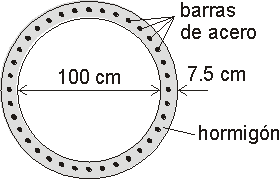
\includegraphics{ej6.pdf}
\end{center}

\dotfill

\begin{quote}
Se puede despreciar el efecto de \textit{Poisson} por las dimensiones. Las tensiones se relacionan por el módulo de \textit{Young}.

\begin{align}
\textit{Hormigón} && \textit{Acero} \nonumber \\
\sigma_{h} &= E_{h}e & \sigma_{a} &= E_{a}e=15E_{h}e \\
\sigma_{h} &= \frac{F_{h}}{A_{h}} & \sigma_{a} &= \frac{F_{a}}{A_{a}}
\end{align}

\begin{minipage}[t]{0.4\linewidth}

Propiedades de las cargas que soporta el hormigón:

\begin{align*}
\frac{F_{h}}{F_{h}+F_{a}}
\end{align*}

\end{minipage} \hfill \begin{minipage}[t]{0.4\linewidth}

Propiedades de las cargas que soporta el acero:

\begin{align*}
\frac{F_{a}}{F_{a}+F_{h}} \\
\end{align*}

\end{minipage}

De (1) y (2) obtengo:

\begin{align*}
F_{h} &= A_{h}E_{h}e & F_{a} &= 15E_{h}A_{a}e
\end{align*}

Evaluando la propiedad para el hormigón:

\begin{align*}
F_{h}+F_{a} &= E_{h}(A_{h}+15A_{a})e & prop_{h} &= \frac{A_{h}}{A_{h}+75A_{a}} \\ \\
A_{a} &= 6.5\cdot 36 & A_{h} &= \left(\frac{100+7.5}{2}\right)^{2}\pi
-\left(\frac{100}{2}\right)^{2}\pi\cdot A_{a}
\end{align*}

\end{quote}

\section*{Apéndice}

\textit{Tensores isotrópicos de rango 0:}

\begin{align*}
Escalares
\end{align*}

\vspace{1em}

\textit{Tensores isotrópicos de rango 1 (sólo el trivial):}

\begin{align*}
A_{i} &= \begin{pmatrix}
0 \\
0 \\
0
\end{pmatrix}
\end{align*}

\vspace{1em}

\textit{Tensores isotrópicos de rango 2:}

\begin{align*}
A_{ij} &= p\delta_{ij}
\end{align*}

\vspace{1em}

\textit{Tensores isotrópicos de rango 3 (isotrópico con respecto a las rotaciones):}

\begin{align*}
A_{ijk} &= \alpha\varepsilon_{ijk}
\end{align*}

\vspace{1em}

\textit{Tensores isotrópicos de rango 4:}

\begin{align*}
A_{ijkl} &= \lambda\delta_{ij}\delta_{kl}
+\mu(\delta_{ik}\delta_{jl}+\delta_{il}\delta_{jk})
+\nu(\delta_{ik}\delta_{jl}-\delta_{il}\delta_{jk})
\end{align*}

\vspace{1em}

\textit{Presión hidrostática:}

\begin{align*}
-p &= \frac{1}{3}\sigma_{rr}
\end{align*}

\begin{thebibliography}{99}
\bibitem{MCF}
Y. C. Fung,
\emph{A First Course in Continuum Mechanics}, 
tercera edición,
PRENTICE HALL,
1994.
\end{thebibliography}

\end{document}